\documentclass[12pt]{article}

% PACKAGES
\usepackage[utf8]{inputenc}
\usepackage[ngerman]{babel}
\usepackage{lmodern}
\usepackage{bookmark}
\usepackage{caption} % Für \caption*{}
\usepackage{siunitx} % SI-Einheiten
\usepackage{mathtools} % Verbessertes "amsmath" (https://de.overleaf.com/learn/latex/Articles%2FMathtools_-_for_beautiful_math)
\usepackage{xcolor}   % Farbiger Text (https://www.overleaf.com/learn/latex/Using_colours_in_LaTeX)
\usepackage{geometry} % Zur Einstellung des Layouts
\usepackage{titlesec} % Einteilung des Inhalts (https://de.overleaf.com/learn/latex/Sections_and_chapters)
\usepackage{fancyhdr} % Für Kopf-/ und Fußzeilen (https://www.overleaf.com/learn/latex/Headers_and_footers)
\usepackage{parskip}
\usepackage{biblatex}
\usepackage{float}


% SETUP
\pagestyle{fancy}
\sisetup{per-mode=fraction, exponent-product = \cdot,separate-uncertainty = true} % Einstellung für siunitx
\addbibresource{VBeispiel.bib}
\geometry{ %A4
  a4paper,
  total = {170mm,240mm},
  left = 20mm,
  top = 30mm
}

% COMMANDS
\newcommand{\uproman}[1]{\uppercase\expandafter{\romannumeral#1}} % Römische Zahlen


% DOC
\begin{document}

% HEADER
\begin{titlepage}
  \centering
  \vspace*{1cm}
  
\includegraphics[width=0.5\textwidth]{Ressourcen/tud_logo_schwarz(RGB)}\\
  \vspace*{0.25cm}
  \large\textmd{Fakultät Physik} \\
  \vspace*{6cm}
  \huge \bfseries AP-2023\_1 - Versuch Beispiel \\
  \vspace*{0.25cm}
  \large Beispielversuch \\
  \vspace*{0.25cm}
  \large\textmd{\href{mailto:tom.engel@tu-dortmund.de}{Tom Engel}} \\
  \large\textmd{\href{mailto:tom.engel@tu-dortmund.de}{Jan Oppoli}} \\
  \vfill
  \small\textmd{Versuch durchgeführt am XX. XXXXXXX 2023}\\
  \small\textmd{Abgabe erstellt am \today}
\end{titlepage}
\tableofcontents
\newpage

\section{Zielsetzung}\label{sec:zielsetzung}
In dem Experiment \ldots

\section{Theorie}\label{sec:theorie}

\begin{figure}[H]
  \centering
  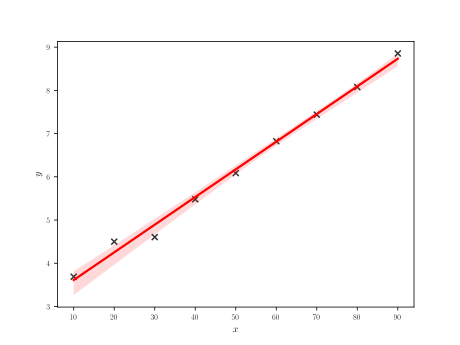
\includegraphics[scale=0.5]{Ressourcen/VBeispiel_plot.svg}
  \caption{Ein Beispiel Plot mit adäquater Beschreibung, einer Quelle und einem Label}\cite{anleitung}\label{fig:1}
\end{figure}

\section{Durchführung}\label{sec:durchfuhrung}
\subsubsection{Aufbau}
\subsubsection{Ablauf}

\section{Auswertung}\label{sec:auswertung}
\subsection{Fehler und Messunsicherheiten}\label{subsec:fehler-und-messunsicherheiten}
Jegliche Fehlerfortpflanzungen und Berechnungen mit Messunsicherheiten finden durch das Python-Package Uncertainties\cite{uncertainties} statt. Somit werden einmal alle bekannten Variablen einmal mit einer speziellen Funktion aus Uncertainties festgelegt. Bei allen nachfolgenden Berechnungen erfolgen die benötigten Fortpflanzungen durch Uncertainties automatisch. Die Formel für die Fehlerfortpflanzung ist 
\begin{align}
  \Delta y=\sum_{i=1}^n\left|\frac{\delta f\left(x_1, \ldots, x_n\right)}{\delta x_i}\right| \Delta x_i.\text{.}\label{gauss}
\end{align}
und die Formel für den Mittelwert/ das arithmetische Mittel ist
\begin{align}
  \bar{x}=\frac{1}{n}\sum_{i=1}^n x_i\label{mittel}
\end{align}
Wie die Ableitungen bestimmt werden ist in der \href{https://readthedocs.org/projects/uncertainties-python-package/downloads/pdf/latest/}{Technischen Dokumentation} selbst nachzulesen.

\section{Diskussion}\label{sec:diskussion}
\newpage

\section{Literaturverzeichnis}\label{sec:literaturverzeichnis}
\printbibliography[heading = none]
\newpage

\section{Anhang}\label{sec:anhang}
\begin{table}[H]
  \centering
  \caption{Beispiel Tabelle mit adäquater Beschreibung}\label{tab:1}
  \begin{tabular}{ll|ll|ll}
      \textbf{T}[$\si{\degreeCelsius}$] & \textbf{p}[$\si{\milli\bar}$] & \textbf{T}[$\si{\degreeCelsius}$] & \textbf{p}[$\si{\milli\bar}$] & \textbf{T}[$\si{\degreeCelsius}$] & \textbf{p}[$\si{\milli\bar}$] \\ \hline
      20 & 55  & 50 & 185 & 80 & 485 \\
      21 & 60  & 51 & 191 & 81 & 500 \\
      \hline
  \end{tabular}
\end{table}
\end{document}
